%%%%%%%%%%%%%%%%%%%%%%%%%%%%%%%%%%%%%%%%%%%%%%%%%%%%
% This will help you in writing your homebook
% Remember that the character % is a comment in latex
%
% 
\chapter{DLX Behaviour}
\label{Summary}

The DLX is a RISC microprocessor able to do basic operations of this category. The purpose of this project is to implement a DLX-like processor, with some additional
characteristics. We start giving a general description of this device and how it works. Then, we will go deep in our project.

\section{Instructions}

Instruction format is on 32 bit and we have a different 6-bit opcode for each one. Depending on this code, we can have 3 different
types of instructions:
 
\paragraph{R-Type:}
For this kind of instruction, the datapath is configured using op-code and func, to make alu register to register operations.\\ 
This type of instructions are characterized by the format:

\begin{figure}[ht]
\centering
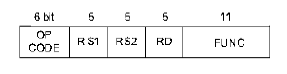
\includegraphics[scale = 0.9]{chapters/figures/rtype} 
\caption{R-Type format}
\label{fig:rtype}  % here is the figure label
\end{figure}

\paragraph{I-Type:}
they are load and store instructions, operations
with immediates or conditional branches.
The format here is:

\begin{figure}[ht]
\centering
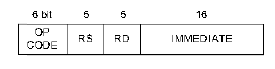
\includegraphics[scale = 0.9]{chapters/figures/itype} 
\caption{I-Type format}
\label{fig:itype}  % here is the figure label
\end{figure}

This operations involve immediates or conditional branches, plus conditional load and store.\\
 
\paragraph{J-Type:}

They are jump instructions and have a format:

\begin{figure}[ht]
\centering
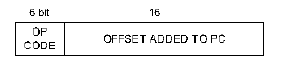
\includegraphics[scale = 0.9]{chapters/figures/jtype} 
\caption{J-Type format}
\label{fig:jtype}  % here is the figure label
\end{figure}

\section{Pipeline}

The pipeline is composed of 5 different stages(Clock Cycles):

\paragraph{Instruction Fetch:}
During this stage the Program Counter is updated, and the corresponding instruction is loaded from the instruction memory 
into the instruction register.

\paragraph{Instuction Decode/Register Fetch:}

The instruction is decoded and registers A,B and IMM are fed by the register file.
 
\paragraph{Execution:}

The values stored in the registers from the previous stage are processed by the alu.
The result is stored into ALUOut register.

\paragraph{Memory Access/Branch Completition:}

Load/Store data from/into the data memory into LMD or coming from ALU. In branches, the PC is replaced with the destination
address in the ALUOut register.  

\paragraph{Write-Back:}
	
Write results into the register file.


\section{Instruction Set}

We implement all the basic DLX instructions, and we add a set of other instructions in order to move our project to pro. The table
1.1 shows the complete Instruction Set.						 


\begin{table}[!htbp]
	\centering
	\begin{tabular}{|c|c|c|c|c|c|c|c|}                                         
	\toprule                                                         
	Mnemonic & Coding & Mnemonic & Coding & Mnemonic & Coding & Mnemonic & Coding\\                                              
	\midrule                                                          
	J		& J,0x02 	& SRAI	& I,0x17	& SLEUI	& I,0x3C	& SGE	& R,0x2D\\                                              
	JAL		& J,0x03 	& SEQI	& I,0x18	& SGEUI	& I,0x3D	& SLTU	& R,0x3A\\                                          
	JR		& J,0x04 	& SNEI	& I,0x19	& SLL	& R,0x04	& SGTU 	& R,0x3B\\						      
	JALR	& J,0x05 	& SLTI	& I,0x1A  	& SRL 	& R,0x06    & SLEU 	& R,0x3C\\                               
	BEQZ 	& B,0x06 	& SGTI 	& I,0x1B  	& SRA 	& R,0x07    & SGEU	& R,0x3D\\                               
	BNEZ 	& B,0x07 	& SLEI 	& I,0x1C  	& ADD	& R,0x20    & MULT	& F,0x0E\\                            
	ADDI	& I,0x08 	& SGEI	& I,0x1D  	& ADDU	& R,0x21	&&				\\     	                            
	ADDUI	& I,0x09 	& LB	& L,0x20  	& SUB	& R,0X23	&&				\\      
	SUBI	& I,0X0A 	& LH	& L,0X21  	& SUBU	& R,0X24	&&				\\      
    SUBUI   & I,0X0B 	& LW	& L,0X23  	& AND  	& R,0X25	&&				\\      
    ANDI    & I,0X0C 	& LBU  	& L,0X24  	& OR 	& R,0X26	&&				\\        
    ORI     & I,0X0D 	& LHU   & L,0X25  	& XOR   & R,0X27	&&				\\    
    LHI		& I,0X0F    & SB  	& S,0X28    & SEQ  	& R,0X28	&&				\\
	XORI    & I,0X0E 	& SH	& S,0X29  	& SNE	& R,0X29	&&				\\      
    SLLI    & I,0X14 	& SW   	& S,0X2B  	& SLT  	& R,0X2A	&&				\\      
    NOP     & N,0X15 	& SLTUI	& I,0X3A  	& SGT	& R,0X2B	&&				\\        
	SRLI	& I,0X16 	& SGTUI	& I,0x3B	& SLE	& R,0x2C	&&				\\										
	\bottomrule                                         
	\end{tabular}                                       
	\caption{Instruction Set}                           
	\label{tableIS} % here is the table label             
\end{table}

\FloatBarrier

\section{Datapath}

Our datapath is divided into 5 different units, each one implementing a pipeline stage. These units are:

\begin{itemize}
\item Fetch Unit;
\item Decode Unit;
\item Execution Unit;
\item Memory Unit;
\item Write-back Unit;
\end{itemize}


\subsection{Pipeline implementation}

The general architecture, including all units, is:

%\begin{figure}[ht]
%\centering
%\includegraphics[]{chapters/figures/datapath} 
%\caption{Datapath schematic}
%\label{fig:datapath}  % here is the figure label
%\end{figure}

Every unit/stage is separated by dashed lines. Stages are connected in cascade, the order is like in the list above. 

\section{Control Unit}

Is the component in advance of send/receive signals from/to datapath in order to manage the instruction flow in the
correct way. We choose to use an hardwired CU, rather than others, because...

\section{Memories}                                      
 We use two RAM as Instruction and Data memories. The IRAM is able to acquire instructions from a compiled .asm file, 
 with the correct coding (see appendix A for the VHDL code).                                            